\chapter{Surveillance clinique}

\section{Données monitorées}

On retrouve à la fois des données mesurées sur le multimètre situé sur
le dessus du module de contrôle et sur le Monitron. Certaines données
sont même affichées aux deux endroits.

\begin{auchum}
\emph{Il est important de noter que pour l'application du protocole de
ventilation du CHUM, c'est toujours les pressions affichées sur le
multimètre du module de contrôle que l'on doit utiliser (moyenne
inspiratoire et moyenne expiratoire).  Les pressions affichées par le Monitron (PEAK PRESSURE et PEEP/CPAP)
sont lues à la crête de l'oscillation et sont par conséquent peu
représentatives des pressions subies par les alvéoles pulmonaires.
}
\end{auchum}

\begin{figure}
	\begin{wide}
	\newcommand{\pexp}{5}
\newcommand{\pins}{18}
\newcommand{\arrpos}{1.06}
\begin{tikzpicture}[
		pressmark/.style={
			draw=gray,
			dashed,
		},
		pline/.style={
			pressmark,
			help lines,
			rounded corners,
			out=0,
			in=180,
			thick
			},
		pcircle/.style={
			pressmark,
			circle,
			inner sep=0.5mm,
			thick
			}
	]

	\begin{axis}[
		width=0.75\textwidth,
		height=5cm,
		name=plot,
		font=\scriptsize,
		try min ticks=6,
		xtick={0,4,8},
		ytick={0,30},
		axis x line=bottom,
		axis y line=middle,
		enlarge y limits={value=0.1, upper},
		enlarge x limits={value=0.05, upper},
		extra y ticks={5, 18},
		extra y tick labels={$P_{ins. moy.}$, $P_{exp. moy.}$},
		extra y tick style={grid=major},
		major grid style={pressmark, thick}
		]

		\addplot [
			black,
			restrict x to domain=0:8,
			] table[x=time, y=Pao] {dat/f300.dat};

		\coordinate (D) at (axis cs: \pgfkeysvalueof{/pgfplots/xmax},\pins);
		\coordinate (B) at (axis cs: \pgfkeysvalueof{/pgfplots/xmax},\pexp);

	\end{axis}

	\pic [opacity=0.99, name=mm, scale=1] at ([xshift=3.2cm, yshift=0cm]plot.east) {multimeter};

		\node [grad] (mmg50) at (mmscreen.north west) {50};
		\node [grad] (mmg0) at (mmscreen.south west) {0};
		\draw [pScale]	(mmg0) -- (mmg50) node [grad, left=0.0mm, pos=0.6, inner sep=0mm] {30};

		\node [below, white, align=left, font=\tiny] at (mmscreen.south) {Percussionaire\\Corporation};

	\node [pcircle] (pmi) at (mmPmi) {\pins};
	\node [pcircle] (pme) at (mmPme) {\pexp};

	\draw [pline] (D) to (pmi);
	\draw [pline] (B) to (pme);
\end{tikzpicture}

	\caption[Pressions affichées sur le multimètre numérique]{La pression inspiratoire moyenne et la pression expiratoire moyenne sont affichées sur me multimètre numérique se trouvant sur le dessus du ventilateur.}
	\end{wide}
\end{figure}
\def\ptitle#1{\vspace{.4\baselineskip}\textbf{#1}\par\vspace{0.4\baselineskip}}

\begin{framed}
	\ptitle{Données affichées par le Multimètre numérique et par le Monitron. }
	\ptitle{Multimètre du module de contrôle }
	\protochum{Pression inspiratoire moyenne}\\
	\protochum{Pression expiratoire moyenne}\\
	Pression moyenne globale\\
	\protochum{Fréquence de percussion ($F_{perc}$)}

	\ptitle{Monitron}
	\raggedright
	Pression inspiratoire de crête\\
	Pression expiratoire de crête (PEP)\\
	Pression moyenne globale\\
	\protochum{Ti (convection)}\\
	\protochum{Te (convection)}\\
	I:E\\
	F\textsubscript{conv}\\
	\protochum{Fréquence de percussion ($F_{perc}$)}\\
	i:e

	\vspace{0.2\baselineskip}
	{\small *\protochum{}\space \emph{Données utilisées dans le
	protocole clinique du CHUM}}
	\end{framed}


\section{Monitorage du rapport \ie}

Il est important de savoir que l'affichage du rapport \ie\ sur le
Monitron n'est fonctionnel que lorsque le Ti est plus petit que le Te.
Lorsque le Ti devient plus grand que le Te (rapport inversé), le
Monitron affiche en permanence 1\string: 1.0.

La meilleure façon de juger du rapport \ie\ est alors d'observer
l'apparence de la courbe de pression sur le monitron.

Les éléments à observer sont:

\begin{itemize}
\item
  Durée du Ti (montée de pression et plateau) versus celle du Te (chute
  de la pression) (observer à 1 ou 2 s par écran);
\item
  Présence d'un plateau. Un plateau où la pression plafonne complètement
		est suggestif d'un ratio inversé. Voir Figure~\ref{figie1}, courbe du bas.
  (observer à 1 ou 2 s par écran);
\item
  Espace sous la courbe de pression. L'augmentation de l'espace sous la
  courbe pendant l'inspiration convective est aussi suggestive d'un
  ratio inversé. Elle témoigne d'une diminution de l'amplitude des
  percussions. Voir Figure~\ref{figie8}, courbe du bas. (observer à 5 ou 8 s par
  écran);
\end{itemize}

\begin{fullwidth}
\begin{figure}
	\def\iehuit{%
\addplot graphics [
	xmin=0,
	ymin=0,
	xmax=1,
	ymax=60
]}

\begin{tikzpicture}

\begin{groupplot}[
		group style={
			group size=1 by 2,
			xlabels at=edge bottom
		},
		enlargelimits=false,
		height=4cm,
		width=\textwidth,
		xtick={0, .25, .5, .75, 1},
		xlabel=Temps (s),
		ylabel=Pression (hPa)
]

\nextgroupplot
\iehuit {img/509-gray.jpg};

\nextgroupplot
\iehuit{img/828-gray.jpg};

\end{groupplot}
\end{tikzpicture}

	\caption[Rapport \ie\ adéquat et inversé (1 s par écran)]{Rapport \ie\ adéquat (en haut) et rapport \ie\ inversé (en
	bas). On observe sur le tracé du bas un Te trop court ne permettant pas
	à la pression de redescendre entre chaque percussion. La pression
	d'équilibre est donc rapidement atteinte à la percussion suivante. Il en
	résulte une faible amplitude de variation de pression à chaque
	percussion. Vitesse de défilement à 1 s par écran.}
	\label{figie1}

	\def\iehuit{%
\addplot graphics [
	xmin=0,
	ymin=0,
	xmax=8,
	ymax=60
]}

\tikzsetnextfilename{fig-ie8}
\begin{tikzpicture}

\begin{groupplot}[
		group style={
			group size=1 by 2,
			xlabels at=edge bottom
		},
		enlargelimits=false,
		height=4cm,
		width=\textwidth,
		xtick={0, 2, 4, 6, 8},
		xlabel=Temps (s),
		ylabel=Pression (hPa)
]

\nextgroupplot
\iehuit {img/329-gray.jpg};

\nextgroupplot
\iehuit{img/629-gray.jpg};

\end{groupplot}
\end{tikzpicture}

	\caption[Rapport \ie\ adéquat et inversé (8 s par écran)]{Rapport \ie\ adéquat (en haut) et rapport \ie\ inversé (en
	bas). On observe une diminution de l'amplitude de percussion sur le
	tracé du bas. Vitesse de défilement à 8 s par écran.}
	\label{figie8}
\end{figure}
\end{fullwidth}

\section{Alarme}\index{alarme}

\subsection{Alarmes du module de contrôle}

\subsubsection*{Alarme du mélangeur air-oxygène}
lbs/po²
Il s'agit d'une alarme pneumatique se déclenchant lorsque le mélangeur
perd son alimentation en air ou en oxygène. Il n'y a pas de fonction
\emph{silence} ou \emph{réarmer~}: l'alarme s'arrête automatiquement
lorsque l'alimentation des deux gaz est rétablie.

\subsubsection{Alarme de surpression}\index{alarme!de surpression}
\tikzsetnextfilename{arlm-surpression}
\knobshow{{}{ALARME DE\\SURPRESSION}}
\marginpar{%
	\centering
	\vspace{\baselineskip}
	\tikzsetnextfilename{btn-raz}
	\begin{tikzpicture}
		\pic [] (PB){pushbutton};
		\node [align=center, font=\scriptsize] at(1,0)  {REMISE\\À ZÉRO};
	\end{tikzpicture}}
Il s'agit d'une alarme pneumatique se déclenchant lors d'une surpression
dans le module de contrôle. Son déclenchement entraine une chute de la
pression délivrée. Une fois la cause corrigée, il faut réarmer l'alarme
(bouton poussoir rouge) pour que la ventilation reprenne normalement.

Au réglage le plus sensible (rotation en sens antihoraire) l'alarme se
déclenche lorsque la pression dans le circuit avoisine les 80 \cmh.

Lorsque cette alarme se déclenche, il faut en premier lieu suspecter un
réglage inadéquat (par exemple fonction \emph{PRESSION DE CONVECTION} ou
\emph{PEP non oscillante} activées ou fréquence de percussion inférieure
à 100) ou une tubulure blanche coincée.

Il est improbable qu'une condition clinique (par exemple toux ou
résistances augmentées) entraine l'activation de cette alarme.

\subsubsection{Alarme de déconnexion}
\index{alarme!de déconnexion}

Il s'agit d'un module indépendant situé sur le côté de l'appareil et
alimenté par une batterie. Cette alarme se déclenche lorsqu'aucune
pression n'est détectée dans le circuit pour une période donnée. Cette
période peut (en théorie\ldots{}) être ajustée au moyen de la roulette
noire.

\subsection{Alarmes du Monitron}

\subsubsection*{Alarme de pression haute}%

Cette alarme se déclenche dès que la pression dans le circuit est
supérieure à la limite réglée. La valeur du réglage est indiquée par une
ligne rouge dans la zone de graphiques.

Son réglage répond même logique que l'alarme de pression haute en
ventilation conventionnelle (par exemple 10 \cmh de plus que la
pression de crête actuelle). Il faut cependant se rappeler que le
déclenchement de l'alarme n'interrompt pas la ventilation étant donné
que le Monitron et le module de contrôle sons indépendants l'un de
l'autre.

\subsubsection*{Alarme de pression basse}

Cette alarme s'active lorsque la pression dans le circuit est inférieure
au seuil réglé pour plus de 6 s (alarme visuelle) et 12 s (alarme
sonore).

Il est à noter qu'une fois la pression rétablie, l'alarme continue à
sonner tant qu'elle n'a pas été réarmée.

\section{Situations particulières}

\subsection{Obstruction de la sonde}\index{obstruction!de la sonde s'intubation}

Étant donné l'absence de monitorage du débit, il est nécessaire de faire preuve
d'une vigilance accrue afin de détecter cette complication. Une obstruction
importante de la sonde peut se manifester par :
		
\begin{itemize}
	\item Une augmentation des pressions de ventilation en l'absence de
	modification des réglages. L'augmentation de la pression à l'inspiration se
	fera de façon plus abrupte, 
	\item Une détérioration des échanges gazeux.
\end{itemize}

La perméabilité de la sonde peut être évaluée en y descendant un cathéter
d'aspiration, que ce soit en cas de doute ou sur une base régulière.  Si
l'abondance des sécrétions est problématique, le ballonnet du tube endotrachéal
peut être partiellement dégonflé pour permettre à celles-ci de remonter dans
l'oropharynx du patient. L'amplitude des percussions devra alors être réajustée
à la hausse pour compenser la fuite créée.

\subsection{Fuite ou déconnexion}\index{fuite}\index{déconnexion}

Une fuite entre le phasitron et le patient ou au niveau du tube endotrachéal se
manifestera par une diminution des pressions mesurées en l'absence de
modification des réglages. La courbe de pression aura une apparence atténuée.
Une fuite dans le circuit d'humidification n’aura pas d'influence sur les
pressions de ventilations. Elle pourra, par contre, modifier la concentration
en oxygène du mélange gazeux administré au patient (appel d’air ambiant),
entrainant une hypoxémie.

\begin{figure}[b]
	\begin{wide}
		\centering
	\begin{tikzpicture}
		\begin{groupplot} [
				group style={
					group size=2 by 1,
					ylabels at=edge left,
				},
				ylabel=$P_{circ.} (hPa)$,
				xlabel=Temps (s),
				width=0.5\textwidth,
				restrict x to domain=1.5:4,
				ymax=40,
				every axis plot post/.style={
					mark=none
				}
			]
			\nextgroupplot [title=Résistances normales]
			\addplot [] table[x=time, y=Pao] {dat/raw5.dat};

		 \nextgroupplot [title=Résistances augmentées]
			\addplot [] table[x=time, y=Pao] {dat/raw15.dat};
		\end{groupplot}
	\end{tikzpicture}

		\caption[Augmentation des résistances]{Modification de l'apparence de
			la courbe de pression suite à une augmentation des résistances.
			Lorsque les résistances sont normales (à gauche), on observe une
			augmentation graduelle des pressions lors de l'inspiration. Cette
			augmentation correspond à l'augmentation de la pression alvéolaire.
			Lorsque les résistances sont élevées, les pressions sont élevées dès
			le début de l'inspiration et restent stable au cours de celle-ci.}
	\end{wide}
\end{figure}

\begin{fullwidth}
\tikzexternaldisable
\begin{exercice}[Calcul du ratio \ie]
	\begin{enumerate}
		\item Sur l'image suivante, au moyen d'une règle:

		\begin{enumerate}
			\item Tracer une ligne sur le début du Ti d'une percussion;
			\item Tracer une ligne sur le début du Te de cette percussion;
			\item Tracer une ligne sur le début du Ti de la percussion suivante;
			\item Mesurer la longueur du Ti et du Te;
		\end{enumerate}

		\item Diviser les deux chiffres par le plus petit des deux, afin
			de ramener à la forme $1:x$ ou $x:1$ \\(voir exemple plus bas).
	\end{enumerate}

	Que remarquez-vous ?

	\centering
	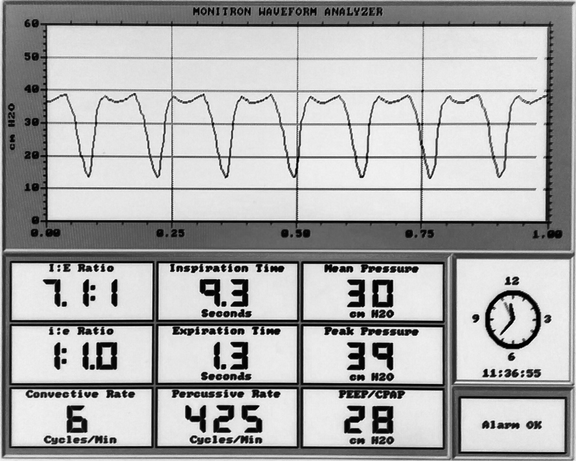
\includegraphics[height=6.5cm]{img/exr-ie-1}

\raggedright	\textbf{Exemple}
	\nopagebreak

\centering
	\begin{tikzpicture}[
				ann/.style={
					line width=1.4pt,
					dashed
				},
				fl/.style={
					<->,
					line width=1.3pt,
					shorten <=0.5mm,
					shorten >=0.5mm,
				},
				meas/.style={
					above=0mm,
					font=\bfseries,
				}
			]
		\node (IMG) {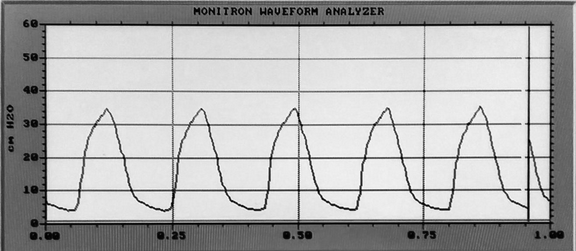
\includegraphics[height=4.8cm]{img/exr-ie-2}};
		\node at (3,.75) [matrix of math nodes, fill=white, rounded corners,
		opacity=0.87, draw=gray]{%
			i:e & =& 9:16\\
						 &=& \frac{9}{9}:\frac{16}{9}\\
						 &=& 1:1,78\\
			};

			\draw [ann](-2.15,-2) -- ++(0,4);
			\draw [ann](-1.6,-2) -- ++(0,4);
			\draw [ann](-.4,-2) -- ++(0,4);

			\draw [fl] (-2.15, 1) -- (-1.6, 1) node [meas, pos=0, anchor=
			east] {9 mm};
			\draw [fl] (-1.6, 1) -- (-0.4, 1) node [meas, pos=1, anchor=west] {16 mm};
	\end{tikzpicture}
\end{exercice}

\tikzexternalenable
\end{fullwidth}
